\documentclass[11pt]{article}
\usepackage[utf8]{inputenc}
\usepackage[T1]{fontenc}
\usepackage[francais]{babel}
\usepackage[francais]{layout}
\selectlanguage{french}

% NE PAS CHANGER !!
\ifx \public \undefined \def\public{etudiants} \fi
\usepackage[\public]{tps}

% Numéro du TP
\newcommand{\numtd}{04}
% Titre du TP
\newcommand{\titretd}{Integers, floats et charsets}

\graphicspath{{imgs/}}

\begin{document}

\entete{\numtd}{\titretd}

\begin{introduction}
 Page web du cours :
 \begin{center}
  \url{http://www.lsv.ens-cachan.fr/~schwoon/enseignement/systemes/ws1617/}
 \end{center}
Ce TP est consacré à des exercices sur les entiers et les nombres à virgule
flottantes. Nous terminerons par aborder les codages de caractères côté
utilisateur. 
\end{introduction}

% {{{ Opérations binaires

\section{Opérations binaires}

Le langage C dispose de mécanismes de manipulation de bits. Par exemple,
considérons deux variables $x$ et $y$ de type entier et l'opérateur $\oplus$
(xor). Notons respectivement $x_i$ et $y_i$ le $i^{ieme}$ bit de $x$ et de $y$.
Le résultat de $x \oplus y$ est le mot $z$ tel que $z_i = x_i \oplus y_i$.

Les opérateurs C sont \& (et), $|$ (ou), \^{ } (xor) et \~{} (not). 

\noindent \textbf{Attention:} ne pas confondre les opérateurs logiques tel que
\&\&, $||$, etc, avec les opérateurs de manipulation des mots binaires. En
effet, là où 4\&2 vaut 0, 4\&\&2 donnera 1.

Les opérations binaires peuvent être condensées ainsi $x=x|2$ peut s'écrire
$x|=2$ et $x=x$\^{ }$y$ peut se noter $x$\^{ }$=y$.

Le langage fournit également les opérateurs de décalage à droite $>>$ ou à
gauche $<<$.

\begin{enumerate}
 \item Étudiez le code suivant où $x$ et $y$ sont des entiers :
\begin{verbatim}
x^=y ; y^=x ; x^=y;
\end{verbatim}
  Détaillez ce que fait ce code.

% {{{ Solution
 \begin{solution}
 Exemple avec $x=5$ et $y=8$.

 \begin{tabular}{ r c c }
  $x=$ & 0101 & 5 \\
  $y=$ & 1000 & 8 \\
  $x\oplus=y$, $x=$ & 1101 & 13 \\
  $y\oplus=x$, $y=$ & 0101 & 5 \\
  $x\oplus=y$, $x=$ & 1000 & 8 \\
 \end{tabular}

 Ce code échange les valeurs de $x$ et d'$y$
\end{solution}
% }}}

 \item Que fait le code suivant :

\begin{verbatim}
 n & (n-1)
\end{verbatim}

% {{{ Solution
\begin{solution}

Supprime le 1 de poids le plus faible (si $n\ne0$). Vaut 0 si $n=0$.

\end{solution}
% }}}

 \item Dans le code suivant $c$ et $n$ sont des entiers :
\begin{verbatim}
for (c = 0; n != 0; n &= (n-1)) c++;
\end{verbatim}
 Quelle valeur prend $c$ en fonction des valeurs de $n$ ?

% {{{ Solution
\begin{solution}

Exemple avec $n=5$.

$c$=0 ; $n$!=0 donc $n$=$n$\&($n$-1) soit 5\&4 101\&100 donc $n$=100 et $c$=1

$n$ est supérieur à 0 donc $n$=4\&3 soit 100\&011 donc $n$=000 et $c$=2

$n$=0

$c$ est le nombre de 1 dans la représentation binaire de $n$.
\end{solution}
% }}}

 \item Proposez les opérations à réaliser pour les fonctions \textit{getBit},
\textit{setBit}, \textit{toggleBit} et \textit{clearBit} prenant chacune deux
arguments $n$, le nombre sur lequel effectuer l'opération, et $p$ la position
du bit à modifier dans $n$ (où 0 est de bit de poids le plus faible). 
\begin{itemize}
 \item \textit{getBit} retourne la valeur du $p^{ième}$ bit de $n$ 
 \item \textit{setBit} passe à 1 la valeur du $p^{ième}$ bit de $n$
 \item \textit{toggleBit} le $p^{ième}$ bit de $n$ passe à son contraire
 \item \textit{clearBit} passe à 0 la valeur du $p^{ième}$ bit de $n$
\end{itemize}

\end{enumerate}

% }}}

% {{{ Séquence de De Bruijn

\section{Trouver le bit de poids le plus faible}

\begin{solution}
Peut-être mentionner à l'orale qu'il existe une méthode triviale
(décaler $x$ à droite et compter jusqu'à ce que $x\&1$ donne 1),
mais cette méthode est de temps $\mathcal{O}(n)$ pour les mots
de longueur $n$. Ou bien, on se crée un tableau qui contient la
solution pour chacun des $2^n$ mots possibles, ce qui rend possible
un lookup en temps constant ($\mathcal{O}(1)$), mais avec un très grand tableau.
Notre méthode prend $\mathcal{O}(1)$ temps et nécessite un tableau
de taille $\mathcal{O}(n)$.
\end{solution}

Dans cette partie nous étudierons une méthode pour efficacement trouver
la position du bit de 1 du poids le plus faible dans un mot binaire.
Soit $x\ne0$ un entier, du coup sa représentation contient au moins un bit de 1.
Par exemple, si la représentation binaire de $x$ est $10011000$, alors le bit
recherché est le 1 suivi par les trois zéros finaux. Dans ce
cas, on note $\ell(x)=3$. L'objectif est de trouver $\ell(x)$ pour un $x\ne0$
donné. On présente cette méthode pour les mots de $2^3=8$ bits, mais elle
peut être généralisée à $2^n$ bits pour n'importe quelle valeur de $n>0$.

La première étape consiste à étudier les séquences dites de \emph{De Bruijn}.
Une séquence de De Bruijn d'ordre $n$ est un mot binaire qui contient
tout mot binaire de longueur $n$.

\begin{enumerate}
\item Combien de mots binaires différents de longueur $n$ existent ?
 Donnez une borne inférieure triviale pour la longueur d'une séquence
 de De Bruijn.

\begin{solution}
Il y a $2^n$ mots différents de longueur $n$. 
Une borne inférieure triviale est de $2^n+(n-1)$, étant donné que chaque mot
de longueur $n$ doit commencer à une position différente et doit être suivi
par $n-1$ bits de plus.
\end{solution}
\end{enumerate}

Un graph de De Bruijn permet de construire des
séquences de De Bruijn. Les sommets du graph d'ordre $n$ sont des chaînes de
$n$ bits. Les sommets $b_1b_2...b_n$ et $c_1c_2...c_n$ sont liés par des
arrêtes dirigées si et seulement si $b_2=c_1,b_3=c_2,...b_n=c_{n-1}$.
Autrement dit, un sommet est lié au suivant en
supprimant son premier bit et en ajoutant un des bits possibles à la fin.
La figure~\ref{DeBruijnOrdre2} page~\pageref{DeBruijnOrdre2} représente
un graph de De Bruijn d'ordre 2.

\begin{figure}[h]
 \centering
 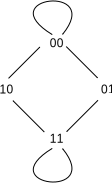
\includegraphics{order-2}
 \caption{\label{DeBruijnOrdre2}Graph de De Bruijn d'ordre 2}
\end{figure}


\begin{enumerate}
\setcounter{enumi}{1}
\item Dessinez le graph de De Bruijn d'ordre 3.

% {{{ Solution

\begin{solution}
\centerline{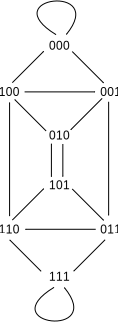
\includegraphics{order-3}}
\end{solution}
\end{enumerate}

% }}}

Une séquence de De Bruijn correspond à un cycle hamiltonien dans
le graph de De Bruijn. Un cycle hamiltonien est un cycle passant uniquement une fois par tous les sommets du graph avant de revenir au point de départ.
On va considérer des cycles commençant et se terminant par le sommet 000.
Par exemple, le seul cycle hamiltonien de
la figure~\ref{DeBruijnOrdre2} page~\pageref{DeBruijnOrdre2} est 00
$\rightarrow$ 01 $\rightarrow$ 11 $\rightarrow$ 10 $\rightarrow$ 00.
Pour obtenir une séquence De Bruijn, il convient de commencer par noter
le sommet initial (00) et les bits rajoutés à la fin de chaque sommet,
ce qui donne, dans ce cas, 00110. On peut
prouver qu'il existe un cycle hamiltonien dans chaque graph de De Bruijn.

\begin{enumerate}
\setcounter{enumi}{2}
\item Trouvez deux séquences de De Bruijn d'ordre 3 en utilisant
le graph dessiné précédemment.  

% {{{ Solution

\begin{solution}

000 $\rightarrow$ 001 $\rightarrow$ 010 $\rightarrow$ 101 $\rightarrow$ 011
$\rightarrow$ 111 $\rightarrow$ 110 $\rightarrow$ 100

0001011100

000 $\rightarrow$ 001 $\rightarrow$ 011 $\rightarrow$ 111 $\rightarrow$ 110
$\rightarrow$ 101 $\rightarrow$ 010 $\rightarrow$ 100

0001110100

\end{solution}
\end{enumerate}

% }}}

Choisissez une séquence de De Bruijn d'ordre 3 que l'on va appeller $s$
par la suite. Si $s$ est composée de bits $b_0b_1b_2\cdots$ et $s'$ une
séquence de longueur 3, on appelle \emph{index} de $s'$ la valeur $i$
telle que $b_ib_{i+1}b_{i+2}=s'$. Par exemple, dans $0001110100$ l'index
de $000$ est de 0 et l'index de $001$ est de 1.

\begin{enumerate}
\setcounter{enumi}{3}
\item Complétez le tableau des indices ci-dessous pour votre séquence $s$.

\begin{center}
 \begin{tabular}{ c | c }
  chaîne & index dans $s$ \\
  \hline
  000 & 0 \\
  001 & \\
  010 & \\
  011 & \\
  100 & \\
  101 & \\
  110 & \\
  111 & \\
 \end{tabular}
\end{center}

% {{{ Solution

\begin{solution}

 En utilisant la séquence 0001011100, on obtient le tableau ci-dessous.
 On observe que la colonne droite est une permutation de $\{0,\ldots,7\}$.

 \begin{center}
  \begin{tabular}{ c | c }
   chaîne & index dans $s$ \\
   \hline
   000 & 0 \\
   001 & 1 \\
   010 & 2 \\
   011 & 4 \\
   100 & 7 \\
   101 & 3 \\
   110 & 6 \\
   111 & 5 \\
  \end{tabular}
 \end{center}
\end{solution}

% }}}

 \item Considérons $0 \leq j < 8 $. En utilisant la séquence $s$ choisie
  précédemment, on considère l'expression suivante :

$e(j):=((s \ll j) \gg 7 ) \mathbin{\&} 7$

Ici, $\ll$ et $\gg$ désignent respectivement un décalage à gauche et un
décalage à droite, et \& est l'opérateur <<et>>.
Quelle est la relation entre $e(j)$ et $j$ ? Est-ce qu'on
peut récupérer $j$ étant donné $e(j)$ ?

\begin{solution}
La relation entre $e(j)$ et $j$ est exactement le tableau établi
précédemment qui est bijectif. Du coup, pour $e(j)=000$
on a $j=0$ etc.
\end{solution}

 \item Quelle valeur donne $x\mathbin{\&}(-x)$
où $-x$ est représenté par complément à deux ?

\begin{solution}
Rappel : le complément à deux est obtenu en inversant les bits de l'écriture
binaire et ensuite ajoutant 1.

Ex : 4 : 00000100 ; complément à 2 : 11111011 ; complément à 2 (+1) : 11111100

Du coup, si la représentation binaire de $x$ est $c_0c_1\cdots c_i10\cdots 0$,
la négation est $\bar{c_0}\bar{c_1}\cdots\bar{c_i}01\cdots 1$, et
la représentation de $-x$ devient $\bar{c_0}\bar{c_1}\cdots\bar{c_i}10\cdots 0$,
et l'expression ci-dessus contient un seul bit de 1, à la position $\ell(x)$,
ce qui vaut $2^{\ell(x)}$.
\end{solution}

 \item Proposez une implémentation de $l(x)$

\end{enumerate}

% }}}

% {{{ Virgule flottante

\section{Virgule flottante}

Rappel : en C, le type \texttt{float} repr\'esente des valeurs r\'eelles
selon le standard IEEE 754 dans la variante de 32 bit, avec 1 bit pour
le signe, 8 pour l'exposant et 23 pour la mantisse. On consid\`ere le
type suivant qui repr\'esente ces composants par trois entiers :

\begin{quote}
\verb+typedef struct { int signe; int exposant; int mantisse; } fc;+
\end{quote}

\begin{enumerate}
\item \'Ecrivez une fonction C qui d\'ecompose un \texttt{float}
  dans ses trois composants. (autrement dit, le param\`etre d'une telle
  fonction est un \texttt{float}, et elle renvoit un \texttt{fc}).
  Par exemple, la représentation en IEEE 754 de 2.5 est :
\begin{quote}
\verb+0 . 1000 0000 . 010 0000 0000 0000 0000 0000+
\end{quote}
Dans ce cas, la structure renvoy\'ee contiendrait $\mathtt{sign}=0$,
$\mathtt{exposant}=0x80=128$ et $\mathtt{mantisse}=0x200000=2097152$.

Rappel : Pour se faire, il convient de se servir de la conversion des
types en C (\emph{typecast}), p.ex., \texttt{(int)f}, o\`u \texttt{f}
est un \texttt{float}, va interpr\'eter le contenu binaire de \texttt{f} comme 
un entier. Assurez-vous d'abord que \texttt{int} a la m\^eme taille
sur votre machine !

\item Cr\'eez une fonction qui fait l'inverse, c'est \`a dire qui renvoie
  le \texttt{float} correspondant \`a une structure \texttt{fc} donn\'ee.

\item R\'ealisez l'addition r\'eelle sur la base de l'addition des entiers,
  en passant par les structures \texttt{fc}. Pour simplifier, on fera les
  restrictions suivantes : (i) les deux op\'erandes sont positifs; (ii)
  on ne traite pas les d\'ebordements, (iii) ni les cas sp\'eciaux NaN/Inf etc.

L'addition dans le type \texttt{fc} se fait en trois \'etapes :
\begin{enumerate}
\item Uniformiser les deux valeurs, c'est \`a dire si les deux exposants sont
  diff\'erents, on ajuste la mantisse d'une des deux selon la
  diff\'erence.
\item Faire la somme des deux mantisses, en tenant compte du bit ``cach\'e''
  repr\'esentant la 1.
\item Normalizer la mantisse pour quelle soit dans $[1,2)$, tout en ajustant
  l'exposant du r\'esultat.
\end{enumerate}

\end{enumerate}



% }}}

% {{{ Codage de caractères

\section{Codage de caractères}

Le codage des caractères est une problématique sensé être résolue par la
généralisation du codage de caractères UTF-8. Malheureusement, de nombreuses
applications anciennes et des machines mal configurées n'utilisent pas ce
standard par défaut. La plupart des éditeurs de textes modernes, tel que vim, et
des terminaux tel que xfce4-terminal que vous utilisez actuellement permettent
de choisir le codage des caractères à utiliser pour l'édition des fichiers. 

La commande \textit{<<file>>} affiche les informations sur un fichier ainsi que
le mode d'encodage utilisé.

Nous allons illustrer le problème d'encodage au travers de l'utilisation du
protocole SMTP définissant les règles d'acheminement des courriels et de la
commande <<telnet>> qui permet d'établir une connexion sur un port donné.

Le protocole SMTP (Simple Mail Transfer Protocol) est ancien et très simple :
\begin{itemize}

 \item une fois un client connecté sur un programme proposant la fonctionnalité
SMTP, le serveur répond avec le code 220 s'il accepte l'établissement de la
connexion ; 

 \item le client se présente via l'instruction <<HELO>> suivit de son nom. Le
serveur valide cette étape par un code 250 ;

 \item le client présente alors l'adresse de l'expéditeur du courriel précédé de
l'instruction <<MAIL FROM: >> auquel le serveur répond une nouvelle fois par un
code 250 (attention, le domaine d'expédition doit exister) ; 

 \item puis l'adresse du destinataire précédé de l'instruction <<RCPT TO: >>
validée par le serveur par un code 250 ; 

\item l'instruction <<DATA>> marque le début du contenu du message qui se
terminera par une ligne ne contenant qu'un point (<<.>>) ;

\item la connexion se termine via l'instruction <<QUIT>>.

\end{itemize}

Assurez-vous que le terminal que vous utilisez est configuré pour l'UTF-8,
envoyez un courriel à votre adresse puis renouveler l'opération avec un
terminal configuré en ISO-8859-1. Observez le résultat et commentez.

% }}}

\end{document}
